\documentclass[zihao=false,fontset=windows]{ctexart}
% ctexart 不接受任意 pt 选项。正文改 {10pt}，方括号里是行距。
\usepackage{scrextend}
\changefontsizes[12pt]{10pt}

\usepackage[a4paper,left=2.35cm,right=2.35cm,top=1.7cm,bottom=1.9cm]{geometry}
\usepackage{xcolor}
\usepackage{graphicx}
\usepackage{amsmath,amssymb}
\usepackage{enumitem}
\usepackage{tabularx}
\usepackage{colortbl}
\usepackage{listings}
\usepackage{hyperref}
\usepackage[most]{tcolorbox}

\definecolor{feishuText}{RGB}{31,35,41}
\definecolor{feishuBlue}{RGB}{36,91,219}
\definecolor{feishuRed}{RGB}{216,57,49}
\definecolor{feishuGray}{RGB}{100,106,115}
\definecolor{feishuGray2}{RGB}{143,149,158}
\definecolor{feishuPinkBg}{RGB}{251,191,188}
\definecolor{quoteBar}{RGB}{51,112,255}
\definecolor{codebg}{RGB}{245,246,247}
\definecolor{codeborder}{RGB}{222,224,227}
\definecolor{inlinebg}{RGB}{242,243,245}
\definecolor{callRed}{RGB}{253,226,226}
\definecolor{callOrange}{RGB}{255,245,235}
\definecolor{callYellow}{RGB}{254,255,240}
\definecolor{callGreen}{RGB}{240,251,239}
\definecolor{callBlue}{RGB}{240,244,255}
\definecolor{callRedSoft}{RGB}{254,241,241}
\definecolor{callSun}{RGB}{255,255,204}
\definecolor{callGreenPage}{RGB}{217,245,214}
\definecolor{tableHead}{RGB}{242,243,245}
\definecolor{tableRule}{RGB}{222,224,227}
\definecolor{codeText}{RGB}{31,35,41}
\definecolor{codeKeyword}{RGB}{0,0,255}
\definecolor{codeComment}{RGB}{0,128,0}
\definecolor{codeString}{RGB}{163,21,21}

\setmainfont{Times New Roman}
\setCJKmainfont{Microsoft YaHei}[AutoFakeBold=2.2]
\setCJKsansfont{Microsoft YaHei}[AutoFakeBold=2.2]
\setCJKmonofont{Microsoft YaHei}[AutoFakeBold=2.2]
\setmonofont{Consolas}
\newfontfamily\emojifont{Segoe UI Emoji}

\hypersetup{
  colorlinks=true,
  urlcolor=feishuBlue,
  linkcolor=feishuBlue,
  unicode=true,
  pdftitle={BLIP-2(2023, Salesforce Research)}
}

\setlength{\parindent}{0pt}
\setlength{\parskip}{0.42em}
\setlength{\fboxsep}{1.5pt}
\setlength{\emergencystretch}{3em}
\linespread{1.28}
\color{feishuText}
\arrayrulecolor{tableRule}
\urlstyle{same}

\setlist[enumerate]{label=\textcolor{feishuBlue}{\arabic*.}, leftmargin=1.7em, itemsep=0.22em, topsep=0.28em, parsep=0.08em, partopsep=0pt}
\setlist[itemize,1]{label=\textcolor{feishuBlue}{\textbullet}, leftmargin=1.35em, itemsep=0.18em, topsep=0.25em, parsep=0.06em, partopsep=0pt}
\setlist[itemize,2]{label=\textcolor{feishuBlue}{◦}, leftmargin=1.45em, itemsep=0.12em, topsep=0.15em}
\setlist[itemize,3]{label=\textcolor{feishuBlue}{\rule[0.18em]{0.38em}{0.38em}}, leftmargin=1.55em, itemsep=0.1em, topsep=0.12em}

\newcommand{\feiEmoji}[1]{{\emojifont #1}}
\newcommand{\incode}[1]{\colorbox{inlinebg}{\ttfamily\small #1}}
\newcommand{\codehead}{{\small\ttfamily\color{feishuGray}代码块}\par\vspace{-0.15em}}
\newcommand{\bigmath}[1]{%
  \begin{center}\large$\displaystyle #1$\end{center}%
}

\lstset{
  language=Python,
  basicstyle=\ttfamily\footnotesize\color{codeText},
  keywordstyle=\color{codeKeyword},
  commentstyle=\color{codeComment},
  stringstyle=\color{codeString},
  showstringspaces=false,
  breaklines=true,
  columns=fullflexible,
  keepspaces=true,
  tabsize=4,
  upquote=true,
  aboveskip=2pt,
  belowskip=0pt,
  xleftmargin=0pt,
  frame=none
}

\tcbset{
  feishubase/.style 2 args={
    enhanced,
    boxrule=0pt,
    arc=8pt,
    left=10pt,
    right=10pt,
    top=7pt,
    bottom=7pt,
    before skip=6pt,
    after skip=6pt,
    colback=#1,
    colframe=#1,
    before upper={\feiEmoji{#2}\hspace{0.45em}\ignorespaces}
  }
}
\newtcolorbox{feishubox}[2]{feishubase={#1}{#2}, breakable}
\newtcolorbox{feishuboxnb}[2]{feishubase={#1}{#2}}
\newtcolorbox{feishucol}{
  enhanced,
  boxrule=0pt,
  arc=0pt,
  colback=white,
  colframe=white,
  left=2pt,
  right=2pt,
  top=1pt,
  bottom=1pt,
  before skip=2pt,
  after skip=2pt
}

\newtcolorbox{feishuquote}{
  enhanced,
  breakable,
  boxrule=0pt,
  leftrule=3pt,
  arc=0pt,
  colframe=quoteBar,
  colback=white,
  left=8pt,
  right=2pt,
  top=2pt,
  bottom=2pt,
  before skip=4pt,
  after skip=4pt,
  before upper=\color{feishuGray}
}

\newtcolorbox{feishucode}{
  enhanced,
  breakable,
  colback=codebg,
  colframe=codeborder,
  boxrule=0.6pt,
  arc=6pt,
  left=6pt,
  right=6pt,
  top=5pt,
  bottom=4pt,
  before skip=6pt,
  after skip=6pt
}

\begin{document}
{\zihao{1}\bfseries BLIP-2(2023, Salesforce Research)\par}

\par\vspace{0.95em}\noindent{\zihao{3}\bfseries 1. 模型结构}\par\vspace{0.28em}

BLIP-2 通过在冻结的预训练图像编码器和冻结的预训练大语言模型之间添加一个轻量级查询 Transformer (Query Transformer, Q-Former) 来对齐视觉和语言模型之间的模态。在整个模型中，Q-Former （\textcolor{feishuRed}{也包括Q-Former之后的MLP}）是\textbf{唯一的可训练模块，而图像编码器和语言模型始终保持冻结状态}。\par

\begin{center}
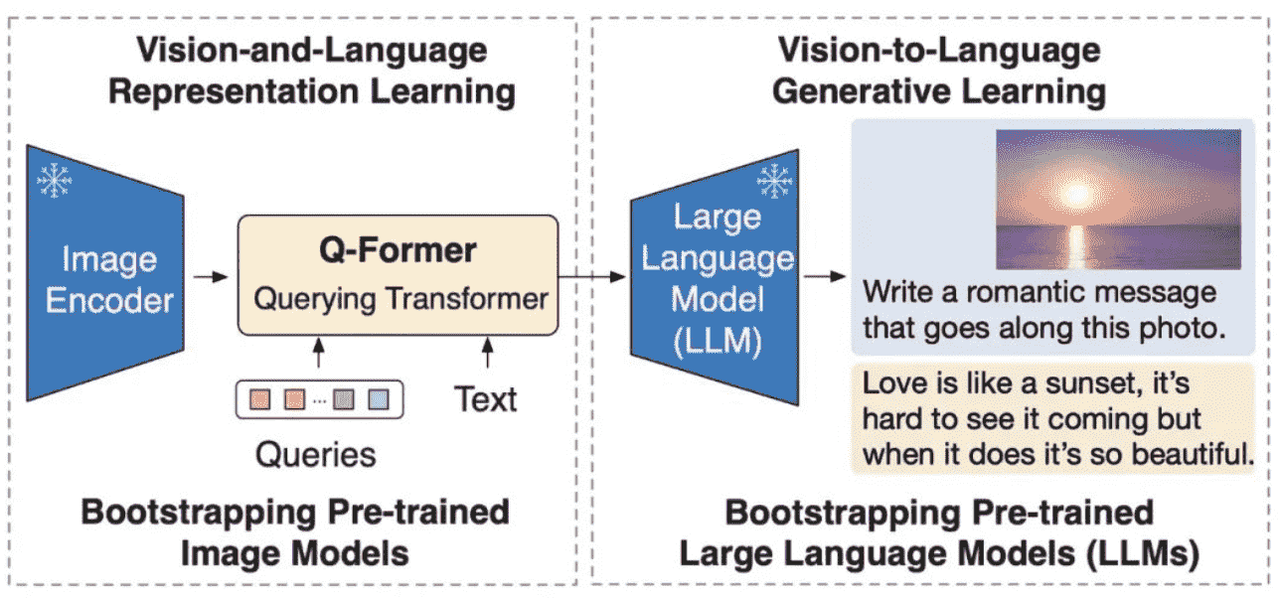
\includegraphics[width=0.98\textwidth]{images/2023-ICML-BLIP-2/fig-01.png}
\end{center}

Q-Former 由两个子模块（双塔）组成，这两个子模块共享相同的自注意力层:\par
\begin{itemize}
\item 与冻结的图像编码器交互的图像 transformer，用于视觉特征提取
\item 文本 transformer（本质就是bert结构），用作文本编码器和解码器
\end{itemize}

\begin{center}
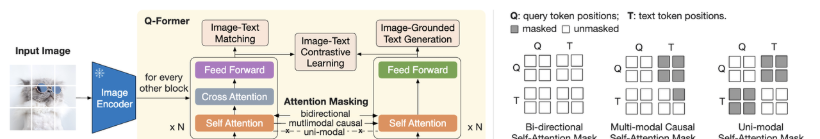
\includegraphics[width=0.98\textwidth]{images/2023-ICML-BLIP-2/fig-02.png}
\end{center}

图像 transformer 从图像编码器中提取固定数量的输出特征。同时，图像 transformer 接收若干查询嵌入作为输入，这些查询嵌入是可训练的。这些查询还可以通过共享的自注意力层与文本进行交互。\par

\begin{feishubox}{callOrange}{📒}
Q-Former 分两个阶段进行预训练。第一阶段，图像编码器被冻结，Q-Former 通过三个损失函数进行训练，\textcolor{feishuRed}{并且使用三个不同的Mask以防止Attention信息泄漏（因为Attention权重是共享的）:}\par
\begin{itemize}
\item Image-Text Contrastive Learning (ITC) loss：这个跟 \href{https://swfvqxo30ma.feishu.cn/wiki/XD9EwE3jRip45RkWXwqciuFWnZd}{CLIP} 是一样的。\textbf{通过对比正例与负例的图文相似度来最大化图像与文本的互信息。}用单模态自注意力屏蔽使得 query 与文本各自独立学习特征，再从多个 query 中选取最高相似度与文本嵌入对齐，从而提升图文对齐能力。
\item Image-Text Matching (ITM) loss：在 ITM 任务中，模型需要通过一个二分类任务\textbf{判断一对图像和文本是否匹配}。\textcolor{feishuRed}{采取的负样本挖掘策略是Albef采用的，即挖掘每一个batch里面，除了正样本外相似度最高的负样本。}样本采用双向自注意力让 query 与文本互相可见，并将所有 query 的输出经过线性分类器后取平均作为匹配分数，同时通过硬负例挖掘强化模型对图文细粒度对齐的判别能力。
\item Image-grounded Text Generation (ITG) loss：\textbf{用于训练 Q-Former 模型在给定输入图像条件下生成文本。}在注意力机制上，queries 之间互相可见但是不能看到文本 token，而文本 token 可以看到所有的 queries 以及它之前的文本 token。此外将 CLS token 替换为 DEC token 以便提示模型进行解码任务。
\end{itemize}
\end{feishubox}

\begin{tcbraster}[raster columns=2, raster equal height=rows, raster column skip=9pt, raster row skip=8pt, raster left skip=0pt, raster right skip=0pt]
\begin{feishucol}
通过第一阶段的训练，Query 已经能够理解图片的含义了，接下来就是让 LLM 也能够理解图片信息，因此作者针对两类不同 LLM 设计了不同的任务：\par
\end{feishucol}
\begin{feishucol}
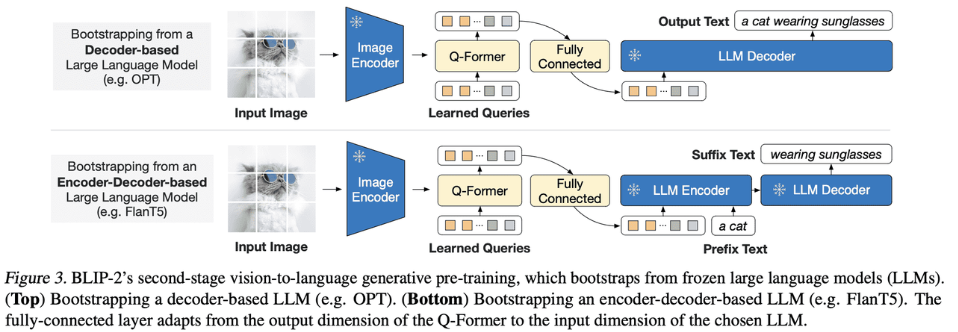
\includegraphics[width=\linewidth]{images/2023-ICML-BLIP-2/fig-03.png}
\end{feishucol}
\end{tcbraster}

\begin{itemize}
\item Decoder 类型的 LLM（如 OPT）：以 Query 做输入，文本做目标；
\item Encoder-Decoder 类型的 LLM（如 FlanT5）：以 Query 和一句话的前半段做输入，以后半段做目标；
\end{itemize}

\textcolor{feishuRed}{因为不同模型的 embedding 维度不同，所以这里还加上了一个全连接层。}\par

\begin{feishubox}{callGreenPage}{🙋}
\textbf{BLIP系列的缺陷点}：\par
作为模态间的连接器来对齐图像和文本，Q-Former并不是一个很好的方案，它使用了image queries来对图像进行抽取，希望基于给定的text prompt来精炼图像信息。但现在从理论和实验角度都证明，这样做实际上是\textcolor{feishuRed}{\textbf{有损压缩}}，这样会导致：\par
\begin{enumerate}
\item 视觉信息不足，不利于细粒度识别任务，比如DocVQA；
\item 有损压缩后，对视觉信息识别不够丰富，会强化模型的幻觉，有时候会按照LLM中的先验知识胡说八道。
\end{enumerate}
\textcolor{feishuRed}{\textbf{作为图像-文本信息的对齐层，Projector使用MLP或者cross attention都会比Q-Former来得更好}}。\par
\end{feishubox}

\par\vspace{0.95em}\noindent{\zihao{3}\bfseries 2. 面试常考细节问题}\par\vspace{0.28em}

看了下网络的代码分析，大多集中在推理端代码分析，而忽略了blip2qformer的训练代码，因此来分析一下：\par

\par\vspace{0.75em}\noindent{\zihao{4}\bfseries Inference（or Train stage-2）}\par\vspace{0.28em}

\begin{center}
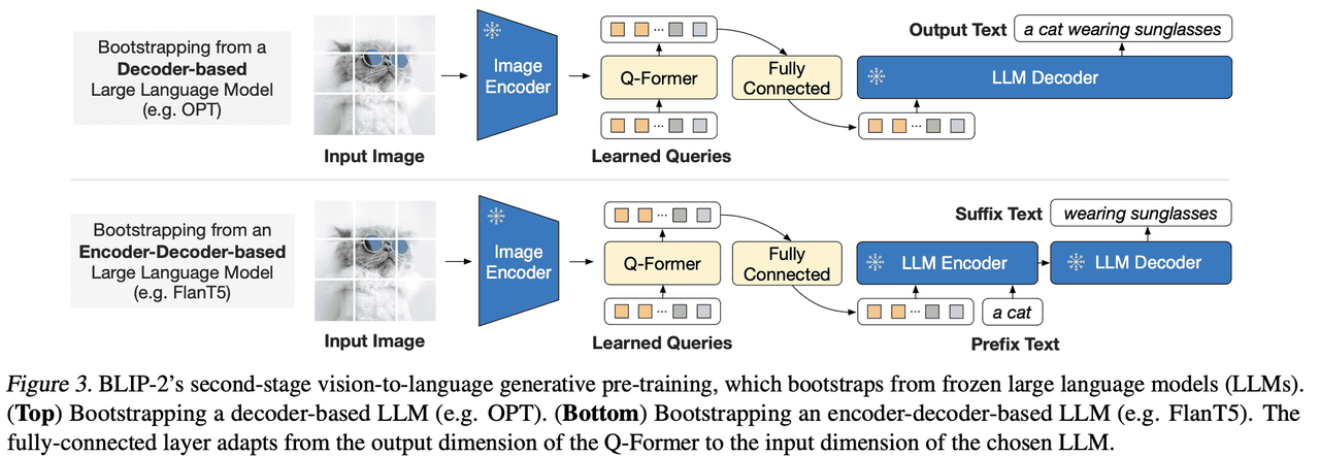
\includegraphics[width=0.98\textwidth]{images/2023-ICML-BLIP-2/fig-04.png}
\end{center}

网络上分析的代码多是推理端的，blip2在做推理的时候，Q-former双塔结构只有图像一侧的block起作用，相对来说流程上是比较简单的，即过N个Blip2QFormerLayer输出的learnable tokens作为图像特征，过mlp之后直接作为大模型输入的前缀embedding，代码及关键注释如下（这个BertLayer即是QformerLayer，下文解释）：\par

\begin{feishucode}
\codehead
\begin{lstlisting}
class BertLayer(nn.Module):
    ...
    def forward(...):
        ...
        # 如果有 query_length，需要对 query tokens 和剩余 tokens 分开处理
        if query_length > 0:
            # 取出前 query_length 个 token 的注意力输出
            query_attention_output = attention_output[:, :query_length, :]
            # 如果存在 cross-attention，就只对 query 部分进行跨注意力
            if self.has_cross_attention:
                ...
                cross_attention_outputs = self.crossattention(
                    query_attention_output,
                    attention_mask=attention_mask,
                    head_mask=head_mask,
                    encoder_hidden_states=encoder_hidden_states,
                    encoder_attention_mask=encoder_attention_mask,
                    output_attentions=output_attentions,
                )
                # cross_attention_outputs[0]: 跨注意力后的 query 部分
                query_attention_output = cross_attention_outputs[0]
            # 对 query 部分做专门的前馈网络 (feed_forward_chunk_query)
            layer_output_query = apply_chunking_to_forward(
                self.feed_forward_chunk_query,  # 针对 query 的前馈网络
                self.chunk_size_feed_forward,
                self.seq_len_dim,
                query_attention_output,
            )
        ...
        # 将最终输出放回 outputs，并加上 present_key_value
        outputs = (layer_output,) + outputs
        outputs = outputs + (present_key_value,)
        return outputs
\end{lstlisting}
\end{feishucode}

\par\vspace{0.6em}\noindent{\zihao{-4}\bfseries Q：为什么 Q-Former 连接到 LLM 需要线性层？}\par\vspace{0.2em}

标准答案是进行维度对齐，因为要适配不同的LLM。\par

\begin{feishuquote}
论文图片上的注脚原文：The fully-connected layer adapts from the output dimension of the Q-Former to the input dimension of the chosen LLM.\par
\end{feishuquote}

但是事实上我觉得这个MLP是起到模态对齐和融合作用的，毕竟qformer提取出的learnable和stage-2的文本信息可能存在分布上的差异。\par

\par\vspace{0.6em}\noindent{\zihao{-4}\bfseries Q：为什么stage-2要放开Q-Former的训练？}\par\vspace{0.2em}

我看到这个问题很多博主是笼统的说“只训练MLP”，其实Qformer是一起训练的，一是参考图片上没有forzen符号；二是可以看blip2opt的代码，是没有frozen qformer的：\par

\begin{feishucode}
\codehead
\begin{lstlisting}
@registry.register_model("blip2_opt")
class Blip2OPT(Blip2Base):
    def __init__(
        ...
    ):
        super().__init__()
        # === 1. 初始化分词器 ===
        self.tokenizer = self.init_tokenizer()

        # === 2. 初始化视觉编码器并视需要冻结 ===
        self.visual_encoder, self.ln_vision = self.init_vision_encoder(
            vit_model,
            img_size,
            drop_path_rate,
            use_grad_checkpoint,
            vit_precision
        )
        if freeze_vit:
            for name, param in self.visual_encoder.named_parameters():
                param.requires_grad = False
            self.visual_encoder = self.visual_encoder.eval()
            self.visual_encoder.train = disabled_train
            logging.info("freeze vision encoder")

        # 3. 初始化 Qformer：不对Qformer做requires_grad=False，所以它是可训练的 
        self.Qformer, self.query_tokens = self.init_Qformer(
            num_query_token, self.visual_encoder.num_features
        )
        self.Qformer.cls = None
        self.Qformer.bert.embeddings.word_embeddings = None
        self.Qformer.bert.embeddings.position_embeddings = None
        for layer in self.Qformer.bert.encoder.layer:
            # 这里是去除文本部分 BERT 的 FFN
            layer.output = None
            layer.intermediate = None

        # === 4. 初始化并冻结 OPT 模型 ===
        self.opt_tokenizer = AutoTokenizer.from_pretrained(opt_model, use_fast=False)
        self.opt_model = OPTForCausalLM.from_pretrained(
            opt_model, torch_dtype=torch.float16
        )
        for name, param in self.opt_model.named_parameters():
            param.requires_grad = False

        # === 5. 投影层 ===
        self.opt_proj = nn.Linear(
            self.Qformer.config.hidden_size, self.opt_model.config.hidden_size
        )

        self.max_txt_len = max_txt_len
        self.prompt = prompt
        prompt_tokens = self.opt_tokenizer(self.prompt, return_tensors="pt")
        self.prompt_length = prompt_tokens.attention_mask.sum(1)

        self._apply_lemmatizer = apply_lemmatizer
        self._lemmatizer = None
\end{lstlisting}
\end{feishucode}

至于为什么要放开Q-Former，我的理解是弥合qformer对齐数据和stage-2的文本数据的分布差异，并且放开qformer会增加灵活性。\par

\par\vspace{0.75em}\noindent{\zihao{4}\bfseries Train（stage-1）}\par\vspace{0.28em}

\begin{center}
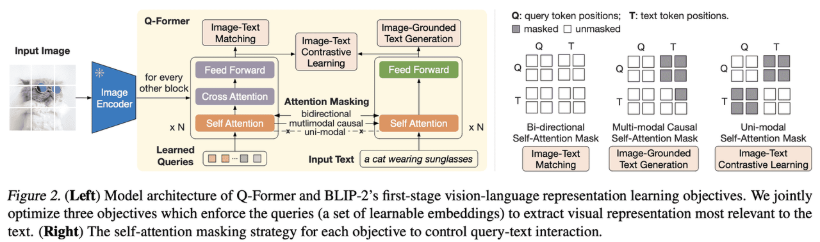
\includegraphics[width=0.98\textwidth]{images/2023-ICML-BLIP-2/fig-05.png}
\end{center}

Qformer的训练（stage-1）会比推理端（or stage-2）要复杂，因为涉及到三个训练任务，我们逐步以QA的形式讲解：\par

\par\vspace{0.6em}\noindent{\zihao{-4}\bfseries Q：ITC、ITM、ITG任务是什么？三个训练任务是怎么安排的？}\par\vspace{0.2em}

这里的三个任务是并列的，没有依赖关系，也没有在ITM上采取hard negtive策略（而是对每一个正样本随机采样一个负样本），最后的loss是三个任务的loss简单加和。\par

\begin{feishucode}
\codehead
\begin{lstlisting}
class Blip2Qformer(Blip2Base):
    def forward(self, samples):
        image = samples["image"]
        text = samples["text_input"]

        # === 视觉编码 ===
        image_embeds = self.ln_vision(self.visual_encoder(image))
        image_atts = torch.ones(image_embeds.size()[:-1], dtype=torch.long).to(image.device)

        query_tokens = self.query_tokens.expand(image_embeds.shape[0], -1, -1)
        query_output = self.Qformer.bert(
            query_embeds=query_tokens,
            encoder_hidden_states=image_embeds,
            encoder_attention_mask=image_atts,
            use_cache=True,
            return_dict=True,
        )
        image_feats = F.normalize(self.vision_proj(query_output.last_hidden_state), dim=-1)

        # === 文本编码 ===
        text_tokens = self.tokenizer(
            text,
            padding="max_length",
            truncation=True,
            max_length=self.max_txt_len,
            return_tensors="pt",
        ).to(image.device)
        text_output = self.Qformer.bert(
            text_tokens.input_ids,
            attention_mask=text_tokens.attention_mask,
            return_dict=True,
        )
        text_feat = F.normalize(self.text_proj(text_output.last_hidden_state[:, 0, :]), dim=-1)

        # ------------------- 1. Image-Text Contrastive (ITC) Loss --------
        image_feats_all = concat_all_gather(image_feats)  # [batch_size*num_gpu, num_query_tokens, embed_dim]
        text_feat_all = concat_all_gather(text_feat)      # [batch_size*num_gpu, embed_dim]
        
        # 相似度计算，聚合 query tokens
        sim_q2t = torch.matmul(image_feats.unsqueeze(1), text_feat_all.unsqueeze(-1)).squeeze()
        sim_i2t, _ = sim_q2t.max(-1)
        sim_i2t = sim_i2t / self.temp

        sim_t2q = torch.matmul(
            text_feat.unsqueeze(1).unsqueeze(1),
            image_feats_all.permute(0, 2, 1)
        ).squeeze()
        sim_t2i, _ = sim_t2q.max(-1)
        sim_t2i = sim_t2i / self.temp

        # 目标索引（正样本）
        rank = dist.get_rank()
        bs = image.size(0)
        targets = torch.linspace(
            rank * bs, rank * bs + bs - 1, bs, dtype=int
        ).to(image.device)

        # 如果有 image_id，就用特殊的 soft label；否则用 cross_entropy
        if "image_id" in samples.keys():
            ...
            loss_itc = (loss_t2i + loss_i2t) / 2
        else:
            loss_itc = (
                F.cross_entropy(sim_i2t, targets, label_smoothing=0.1)
                + F.cross_entropy(sim_t2i, targets, label_smoothing=0.1)
            ) / 2

        # ------------------- 2. Image-Text Matching (ITM) Loss -----------
        ...
        output_itm = self.Qformer.bert(
            text_ids_all,
            query_embeds=query_tokens_itm,
            ...
            encoder_hidden_states=image_embeds_all,
            ...
        )
        vl_embeddings = output_itm.last_hidden_state[:, : query_tokens_itm.size(1), :]
        vl_output = self.itm_head(vl_embeddings)
        logits = vl_output.mean(dim=1)

        itm_labels = torch.cat(
            [torch.ones(bs, dtype=torch.long), torch.zeros(2 * bs, dtype=torch.long)],
            dim=0,
        ).to(image.device)
        loss_itm = F.cross_entropy(logits, itm_labels)

        # ------------------- 3. Language Modeling (LM) Loss -------------
        decoder_input_ids = text_tokens.input_ids.clone()
        decoder_input_ids[:, 0] = self.tokenizer.bos_token_id
        labels = decoder_input_ids.masked_fill(decoder_input_ids == self.tokenizer.pad_token_id, -100)

        lm_output = self.Qformer(
            decoder_input_ids,
            attention_mask=torch.cat(
                [
                    torch.ones(query_tokens.size()[:-1], dtype=torch.long).to(image.device),
                    text_tokens.attention_mask
                ],
                dim=1
            ),
            past_key_values=query_output.past_key_values,
            return_dict=True,
            labels=labels,
        )
        loss_lm = lm_output.loss

        # ------------------- Total Loss -------------------
        return BlipOutput(
            loss=loss_itc + loss_itm + loss_lm,  # 总损失
            loss_itc=loss_itc,
            loss_itm=loss_itm,
            loss_lm=loss_lm,
        )
\end{lstlisting}
\end{feishucode}

\par\vspace{0.6em}\noindent{\zihao{-4}\bfseries Q：ITM任务的负样本挖掘策略？}\par\vspace{0.2em}

\textcolor{feishuRed}{采取的负样本挖掘策略是ALBEF采用的，即挖掘每一个batch里面，除了正样本外相似度最高的负样本。}\par

原始一个Batch里面正样本对的数量为 BatchSize\par

对于负样本图片：找出 \textbf{原始图片} 与 \textbf{最难区分的图片 }拼接\par

对于负样本文本：找出 \textbf{原始文本} 与 \textbf{最难区分的文本} 拼接\par

因为负样本需要找到每个样本对应最难区分的负样本，然后与原始样本拼接，这样负样本的批次就是原始批次的两倍，为：2 x BatchSize。\par

这也解释了为什么ITM任务的label代码是：\par

\begin{feishucode}
\codehead
\begin{lstlisting}
itm_labels = torch.cat(
    [torch.ones(bs, dtype=torch.long), torch.zeros(2 * bs, dtype=torch.long)],
    dim=0,
).to(image.device)
\end{lstlisting}
\end{feishucode}

\par\vspace{0.6em}\noindent{\zihao{-4}\bfseries Q：在代码上的Qformer是怎么实现的？共享Self-Attention是怎么实现的？}\par\vspace{0.2em}

Qformer是一个特殊修改后的bert模型，即加上一个Cross Attention模块和FFN，如下即是一个Qformer：\par

\begin{feishucode}
\codehead
\begin{lstlisting}
class BertLMHeadModel(BertPreTrainedModel):

    _keys_to_ignore_on_load_unexpected = [r"pooler"]
    _keys_to_ignore_on_load_missing = [r"position_ids", r"predictions.decoder.bias"]

    def __init__(self, config):
        super().__init__(config)

        self.bert = BertModel(config, add_pooling_layer=False)
        self.cls = BertOnlyMLMHead(config)

        self.init_weights()
        ......
\end{lstlisting}
\end{feishucode}

而具体Cross Attention模块和FFN的添加体现在魔改的bert layers上：\par

\begin{feishucode}
\codehead
\begin{lstlisting}
class BertLayer(nn.Module):
    def __init__(self, config, layer_num):
        super().__init__()
        self.config = config
        self.chunk_size_feed_forward = config.chunk_size_feed_forward
        self.seq_len_dim = 1
        self.attention = BertAttention(config)
        self.layer_num = layer_num
        if (
            self.config.add_cross_attention
            and layer_num % self.config.cross_attention_freq == 0
        ):
            self.crossattention = BertAttention(
                config, is_cross_attention=self.config.add_cross_attention
            )
            self.has_cross_attention = True
        else:
            self.has_cross_attention = False
        self.intermediate = BertIntermediate(config)
        self.output = BertOutput(config)

        self.intermediate_query = BertIntermediate(config)
        self.output_query = BertOutput(config)
\end{lstlisting}
\end{feishucode}

这个bert layer特殊的地方在于有一个cross attention层，以及两个FFN；\par

\par\vspace{0.6em}\noindent{\zihao{-4}\bfseries Q：Qformer内部特征的维度是怎么对齐的？}\par\vspace{0.2em}

全部hidden\_dim设为vision的dim，从而实现统一。\par

\begin{feishucode}
\codehead
\begin{lstlisting}
......
def init_Qformer(cls, num_query_token, vision_width, cross_attention_freq=2):
        encoder_config = BertConfig.from_pretrained("bert-base-uncased")
        encoder_config.encoder_width = vision_width
        # insert cross-attention layer every other block
        encoder_config.add_cross_attention = True
        encoder_config.cross_attention_freq = cross_attention_freq
        encoder_config.query_length = num_query_token
        Qformer = BertLMHeadModel.from_pretrained(
            "bert-base-uncased", config=encoder_config
        )
        ......
\end{lstlisting}
\end{feishucode}

\par\vspace{0.6em}\noindent{\zihao{-4}\bfseries Q：Blip-2使用的ViT特征是哪一层的？}\par\vspace{0.2em}

是倒数第二层的特征：We remove the last layer of the ViT and uses the second last layer’s output features, which leads to slightly better performance.\par

\end{document}
